\documentclass[a4paper,11pt,utf8]{scrartcl}

\usepackage[ngerman]{babel}
\usepackage[utf8]{inputenc}
\usepackage[a4paper, left=2cm, right=2cm, top=1.5cm, bottom=1.5cm]{geometry}
\usepackage{graphicx}
\usepackage{stmaryrd}
\usepackage{listings}
\usepackage{amsmath}
\usepackage[hidelinks]{hyperref}
\usepackage[onehalfspacing]{setspace}
\usepackage{listings}
\usepackage{color}
\usepackage{tikz}
\usepackage{enumitem}

\usetikzlibrary{shapes,arrows}

\definecolor{dkgreen}{rgb}{0,0.6,0}
\definecolor{gray}{rgb}{0.5,0.5,0.5}
\definecolor{mauve}{rgb}{0.58,0,0.82}

\lstset{frame=tb,
  aboveskip=3mm,
  belowskip=3mm,
  showstringspaces=false,
  columns=flexible,
  basicstyle={\small\ttfamily},
  numbers=none,
  numberstyle=\tiny\color{gray},
  keywordstyle=\color{blue},
  commentstyle=\color{dkgreen},
  stringstyle=\color{mauve},
  breaklines=true,
  breakatwhitespace=true,
  tabsize=3
}

\setlength{\headsep}{.5cm}

\begin{document}

\pagestyle{empty}

% Titlepage
\noindent
Wissens- und Content-Management \hfill Simon Hüning \hfill \today\vspace{-.4cm}\\
\begin{center}
\huge\textsf{Lösungsskizze}\vspace{.1cm}\\
\large Erstellung neuer geographischer Routen anhand von existierenden Routen
\end{center}

\section{Projektbeschreibung}

Ziel dieses Projektes ist es, eine Webanwendung zu entwickeln, die eine soziale Plattform bietet, um Touren mit anderen Leuten zu planen, neue Routen zu erstellen und diese zu bewerten. Kern dieser Anwendung soll ein Algorithmus sein, der auf der Basis schon bestehender Routen automatisch oder manuell eine neue Route berechnen und hinzufügen soll. 

Die Anwendung teilt sich in folgende Komponenten auf:

\begin{itemize}
	\item Import-/Export-Funktionalität
	\item soziale Komponente
		\begin{itemize}[label=$\bullet$]
			\item Benutzerverwaltung
			\item Forum
			\item Bewertungsfunktion
			\item \dots{}
		\end{itemize}
	\item Persistenz der Routen
	\item Sammeln von Routen
	\item Berechnung neuer Routen
	\item Visualisierung der Routen
\end{itemize}

Da die Entwicklung aller Komponenten wahrscheinlich den Zeitrahmen dieser Veranstaltung überschreiten würde und dieses Projekt als \textit{Proof-of-Concept} dienen soll, wird die \glqq soziale Komponente\grqq{} im Rahmen der Ausarbeitung außen vor gelassen.

\section{Installation}

Damit die Anwendung kompilations- und lauffähig ist, müssen folgende Programme vorinstalliert sein:

\begin{itemize}
	\item Java 8 JDK\footnote{\url{http://www.oracle.com/technetwork/java/javase/downloads/jdk8-downloads-2133151.html}}
	\item PostgresSQL 9.6.1\footnote{\url{https://www.postgresql.org}}
	\item PostGIS 2.3.1 \footnote{\url{http://postgis.net/}}
	\item Eclipse Neon mit Maven-Plugin \footnote{\url{https://eclipse.org/downloads/packages/eclipse-ide-java-ee-developers/neon3}}
	\item WildFly 10.1 Application Server\footnote{\url{http://wildfly.org/}}
\end{itemize}

Die Quelldateien können unter \url{https://github.com/simhue/wisscontmgmtprak} heruntergeladen werden. Zunächst muss in der Datenbank das Schema angelegt werden. Das dazugehörige SQL-Skript liegt unter \texttt{sql\textbackslash{}createdb.sql}. Im Skript müssen ggf. noch Benutzer und Datenbankname angepasst werden. 

Sobald das Schema angelegt ist, kann der \textit{TourenCrawler} kompiliert und gestartet werden. Dazu müssen der \textit{TourenCrawler} und \textit{TourenComputer} in Eclipse als Maven-Projekte hinzugefügt werden. 

\begin{enumerate}
	\item Eclipse starten und neuen Workspace anlegen
	\item File $\rightarrow$ Import $\rightarrow$ Maven $\rightarrow$ Existing Maven Projects  Ordner auswählen in dem die Projekte liegen
	\item Projekte auswählen und hinzufügen
	\item Im TourenCrawler-Projekt die Datei \texttt{config.properties} öffnen und die Datenbankdaten eintragen.
	\item Rechtsklick auf TourenCrawler-Projekt $\rightarrow$ Run As... $\rightarrow$ Java Application
	\item \texttt{de.unileipzig.contentmanagement.praktikum.Crawler} aus der Liste Auswählen und Ok drücken
\end{enumerate}

Jetzt wird der \textit{TourenCrawler} gestartet und er importiert 100 Strecken in die Datenbank.

Damit der \textit{TourenComputer} eine Verbindung mit der Datenquelle aufbauen kann, müssen die Verbindungsdaten im WildFly hinterlegt werden.\footnote{\url{https://yellowshoes.de/2015/01/05/wildfly-jdbc-treiber-und-datasource-einrichten/}} Darauf achten, dass der JNDI-Name der Verbindung \texttt{java:/PostgresDS} gespeichert wird.

Bevor der \textit{TourenComputer} gestartet werden kann, muss der der Schlüssel für die GoogleMaps-API\footnote{\url{https://developers.google.com/maps/documentation/javascript/get-api-key?hl=de}} noch in die Konstante \texttt{G\_MAPS\_KEY} der Klasse \texttt{de.contmgmt.praktikum.MapBean} eingetragen werden. Wenn das erledigt ist, kann der \textit{TourenComputer} als Server-Anwendung gestartet werden (Rechtsklick auf \textit{TourenComputer}-Projekt $\rightarrow$ Run As $\rightarrow$ Run on server). Ggf. muss hier noch der WildFly-Server als Server hinzugefügt werden.\footnote{\url{http://www.mastertheboss.com/jboss-server/wildfly-8/configuring-eclipse-to-use-wildfly-8}} Sobald die Webanwendung gestartet wurde, kann der \textit{TourenComputer} unter \url{http://localhost:8080/MotorcycleTouringComputer/} aufgerufen werden.
 
\section{TourenCrawler}
Um eine Grundlage zu bieten, damit ein neue Strecke berechnet werden kann, müssen vorerst existente Routen von anderen Plattformen gesammelt und in der Datenbank abgelegt werden. Als Basis dient eine Auswahl von Strecken im \texttt{KML}\footnote{\url{https://de.wikipedia.org/wiki/Keyhole_Markup_Language}}-Format der Zeitschrift \textit{MOTORRAD}\footnote{\url{http://maps.motorradonline.de/}}. Die Strecken https://www.postgresql.org/download/werden vom \textit{TourenCrawler} iterativ heruntergeladen, vom \texttt{KML}-Format in das Datenbankschema überführt und anschließend abgespeichert. In diesem Vorgang werden \texttt{KML}-Dokumente, die keine Koordinate enthalten verworfen.

Da die Routen manuell von Nutzern angelegt wurden, sind einige Strecke mangelhaft. Das kann bedeuten, dass GPS-Koordinaten abseits von befahrbaren Straßen hinzeigen oder dass eine Folge von GPS-Koordinaten nur approximativ einen Straßenverlauf widerspiegelt. Ein ungefährer Straßenverlauf beeinträchtigt die Qualität der Route, wenn zwei aufeinanderfolgende Koordinaten eine bestimmte Entfernung zueinander überschreiten. Durch diese \glqq Lücke\grqq{} ist unklar, wo die eigentliche - vom Autor gewollte - Strecke entlangführen soll. Das macht eine mögliche automatische Angleichung schwierig, da interessante Teilabschnitte der Strecke übersprungen werden könnten. 

Auch ist es herausfordernd, eine legitime Maximalentfernung zwischen zwei Koordinaten zu finden. Eine Idee war, dass sich die Qualität einer Strecke anhand der Anzahl der Koordinaten relativ zur Gesamtlänge der Route berechnen lässt. Dafür wurde mit Hilfe der \textit{PostGIS}-Stored-Function \texttt{ST\_Length(linestring)}\footnote{\url{https://postgis.net/docs/ST_Length.html}} die Länge von 898 Strecken ermittelt und daraus die ungefähre durchschnittliche Entfernung $296 m$ berechnet. Ein Überschreiten dieses Durchschnittswertes wurde als Ausschlusskriterium genommen. Bei Betrachtung des Ergebnisses des Testimports fiel auf, dass ein Großteil der Strecken verworfen und unsaubere Strecken nicht gefiltert wurden. Da die \glqq Lücken\grqq{} vereinzelt in sonst fehlerlosen Strecken auftreten können, muss jeder Koordinatenpunkt $p_i$ mit dem folgenden Punkt $p_{i+1}$ bzw. die Entfernung der beiden Punkte zueinander verglichen werden\footnote{\texttt{ST\_Distance(p1, p2)} \url{https://postgis.net/docs/ST_Distance.html}}. Nach Auflistung der größten Entfernungen lies sich $1500 m$ als akzeptabler Grenzwert festlegen. Die größere Entfernung verhindert, dass Strecken verworfen werden die willentlich längere Geraden enthalten (z.B. eine gerade Landstraße oder Autobahn). Dieser Ansatz hat sich als der erfolgreichere Filter herausgestellt und wird weiterhin als solcher genutzt.

\section{TouringComputer}
\subsection{Visualisierung der Routen}
Zur Visualisierung wird das \textit{PrimeFaces}\footnote{\url{https://www.primefaces.org/}}-Framework in der Community-Edition benutzt. Das Framework ermöglicht eine einfache Realisierung von einem responsiven Design und bietet eine Schnittstelle zu der \textit{GoogleMaps}-API\footnote{\url{https://developers.google.com/maps/?hl=de}}. Damit die Anwendung einen Ausgangspunkt hat, muss dieser als erstes gesetzt werden. Entweder kann der Benutzer einen Punkt auf der Karte anklicken oder er gibt eine Adresse in das Feld  \glqq Von\grqq{} ein und klickt auf den Setzen-Button. Bei der zweiten Option wird die Adresse mittels \textit{GeoCoding}\footnote{\url{https://developers.google.com/maps/documentation/javascript/geocoding?hl=de}} der GoogleMaps-API in eine geographische Koordinate überführt und auf der Karte dargestellt. 

Nachdem ein Startpunkt selektiert wurde, muss noch ein Umkreis ausgewählt werden in dem Routen dargestellt werden sollen. Dafür gibt der Nutzer eine Kilometer- oder Meilenanzahl an - die Einheit kann ausgewählt werden - und klickt auf den Suchen-Button. Im Folgenden wird eine SQL-Anfrage an die Datenbank gesendet. Die Ergebnismenge der Anfrage enthält alle geografischen Objekte, die sich innerhalb eines Umkreises um den gesetzten Punkt befinden.
\begin{lstlisting}[language=sql]
SELECT route.id, route.description, points.id, points.point FROM route 
	JOIN routepoints ON route.id = routepoints.routeid 
	JOIN points ON routepoints.pointid = points.id 
	WHERE ST_DistanceSphere(point, ST_MakePoint(longitude, latitude)) <=  radius * distanceUnit
	ORDER BY route.id, points.id
\end{lstlisting}

Diese SQL-Anfrage ist auch der Grund warum entschieden wurde, dass jede Koordinate einer Route einzeln als Punkt in die Datenbank abgelegt wird und nicht gesammelt als \textit{LineString}-Objekt\footnote{gezogene Linie entlang der Reihenfolge der inkludierten Punkte}. Da die Umkreisabfrage alle geometrischen Objekte zurückgibt, würden das Resultat \textit{LineStrings} als Ganzes enthalten. Das bedeutet, dass auch Punkte außerhalb des Radius zurückgegeben werden. Die Stored-Function \texttt{ST\_DumpPoints} gibt eine Liste aller Punkte innerhalb eines geometrischen Objektes zurück, jedoch ist dann nicht gewährleistet, dass die Punkte in der Reihenfolge aufgelistet werden, wie sie im \textit{LineString} definiert sind. Die einzelnen Punkte in der Datenbank können anhand der automatisch inkrementierten ID auf- oder absteigend geordnet werden.

Die Resultate werden in entsprechende POJOs geladen. Jede Route wird als \textit{LineString} in das GoogleMaps-Modell hinzugefügt, damit dieses die Routen als anzeigen kann. Jede Route wird dabei anders farblich kenntlich gemacht, damit der Benutzer die einzelnen Strecken visuell unterscheiden kann. Zur besseren Erkennung eines Streckenverlaufs kann jede Strecke angeklickt werden. Darauf wird die Transparenz der Strecke aufgehoben und die Strecke hebt sich deutlich von den anderen ab.

\begin{figure}[htb]
    \centering
    \begin{minipage}[t]{0.45\linewidth}
        \centering
        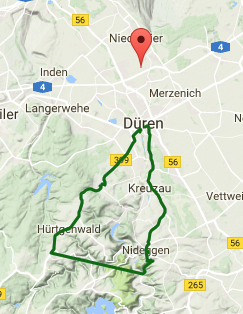
\includegraphics[width=\linewidth]{pics/abgehackt.PNG}
        \caption{$20km$ Umkreis}\label{fig1}
    \end{minipage}% <- sonst wird hier ein Leerzeichen eingefügt
    \hfill
    \begin{minipage}[t]{0.45\linewidth}
        \centering
        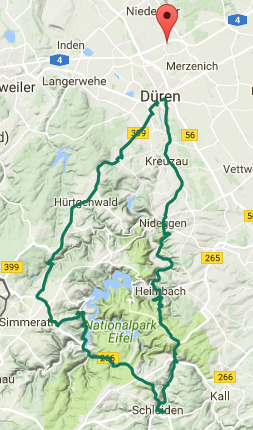
\includegraphics[width=\linewidth]{pics/nichtabgehackt.PNG}
        \caption{$200km$ Umkreis}\label{fig2}
    \end{minipage}
\end{figure}

Dadurch dass Punkte außerhalb des Betrachtungsradius ignoriert werden, treten \glqq Lücken\grqq{} auf, wie sie im \textit{TourenCrawler}-Kapitel beschrieben wurden (s. Abb. \ref{fig1}). Hier ist es schwieriger eine Maximalentfernung zu definieren wie beim Importvorgang, da dort die Routen manuell angelegt wurden und es wahrscheinlicher ist, dass längere Geraden gewollt sein können. Das Angleichen der Gerade an Straßenverläufe durch die \textit{SnapToRoads}-Funktion der \textit{Google-Roads}-API ist problematisch, da diese API am Effektivsten funktioniert, wenn zwei Punkte nahe zueinander sind.\footnote{\url{https://developers.google.com/maps/documentation/roads/snap?hl=de\#demo}} Jedoch wird in der Dokumentation der API nicht genau erläutert, welche Entfernung optimal ist. Da die ID's der Punkte innerhalb einer Route beim Speichern inkrementiert werden, ist die Differenz der ID's von zwei aufeinanderfolgenden Punkten stets $1$. Eine größere Differenz deutet darauf hin, dass Punkte der eigentlichen Route, wie sie in der Datenbank abgespeichert wurde, nicht innerhalb des Suchgebiets befinden. Wenn das der Fall ist, handelt es sich hier um eine Lücke. Dieser Ansatz ist unabhängig von der Länge der Lücke. Die Gesamtroute kann man nun zwischen den Endpunkten der Lücke aufteilen und diese Route als zwei separate Routen behandeln. Es muss noch untersucht werden, ob der Ansatz in der Praxis wie erwartet funktioniert.

\subsection{Routenberechnung}
\begin{figure}[htb]
    \centering
    \begin{minipage}[t]{0.45\linewidth}
        \centering
        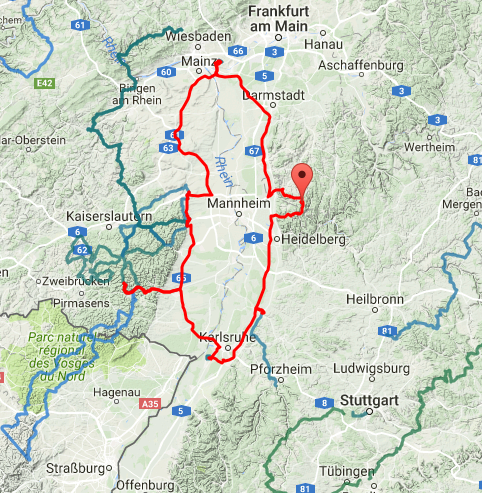
\includegraphics[width=.75\linewidth]{pics/create.PNG}
        \caption{In Rot: neue Streckensegmente}\label{fig3}
    \end{minipage}% <- sonst wird hier ein Leerzeichen eingefügt
    \hfill
    \begin{minipage}[t]{0.45\linewidth}
        \centering
        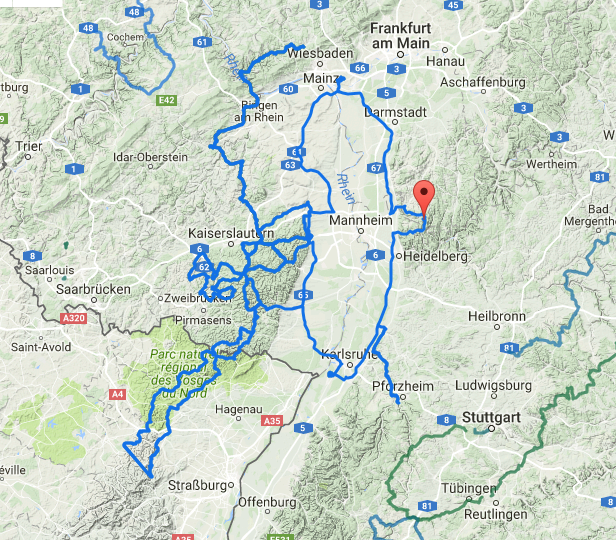
\includegraphics[width=\linewidth]{pics/neu.PNG}
        \caption{Hervorgehoben: neue gespeicherte Route}\label{fig4}
    \end{minipage}
\end{figure}

Der Algorithmus der Routenberechnung nimmt vorher gesetzten Startpunkt als Ausgangspunkt. Die Endpunkte jeder Route im Suchkreis werden gesammelt und mit Hilfe von \texttt{ST\_ClosestPoint} wird der geografisch naheliegendste Punkt aus der Menge zurückgegeben. Durch die GoogleMaps-API wird eine neue Teilstrecke zwischen diesem und dem Startpunkt berechnet. Die neue Teilstrecke wird der neuen Gesamtstrecke als erstes Segment hinzugefügt und der Startpunkt, der auch gleichzeitig das Ende der gesamten Route sein soll, wird der Menge hinzugefügt. Darauf wird die Strecke des Endpunktes ebenfalls hinzugefügt. Der zweite Endpunkt der Strecke wird als neuer Ausgangspunkt gesetzt. Die bisher benutzten Punkt (Startpunkt und die Endpunkte der naheliegendsten Strecke) werden aus der gesammelten Menge entfernt. Mit dem neuen Ausgangspunkt wird der Vorgang wiederholt bis der Zielpunkt (gleich dem Startpunkt) als naheliegendster Punkt zurückgegeben wird.

Dem Benutzer werden die neuen Teilsegmente als rote Linien präsentiert (Abb. \ref{fig3}). Ist der Benutzer mit dem Resultat zufrieden, kann er die neue Strecke speichern, anschließend auswählen und als \texttt{KML}-Dokument exportieren.

\section{Fazit und Ausblick}
Die Webanwendung befindet sich noch im frühen Status der Entwicklung, jedoch bietet die Anwendung eine gute Basis für eine soziale Plattform in der sich Menschen über gemeinsame Touren austauschen können. Die Entwicklung hat gezeigt, dass es möglich ist aufgrund bestehender Routendaten eine neue Strecke berechnen zu lassen. Wegen der prototypischen Implementation des \textit{TourenComputers} wurden nur die Endpunkte einer jeden gefundenen Route im Suchkreis als Zielpunkte für die \textit{GoogleMaps}-Routenberechnung benutzt. Ein Ziel ist es, dass jede Koordinate einer Route als Anker benutzt werden kann. Daraus ergeben sich dann für die weitere Berechnung mehrere Optionen, da der weitere Verlauf der Ankerroute nun in zwei Richtungen weitere gehen kann. Entweder könnte man den Verlauf in beide Richtungen folgen und dem Benutzer mehrere Ergebnisse anbieten oder man nimmt jeweils nur eine Richtung (z.B. die Richtung des kürzen oder längeren Teilstücks).

Auch sollen noch weitere Filteroptionen für die Routenberechnung hinzugefügt werden. So soll der Benutzer zum Beispiel auswählen können, dass nur Strecken im Suchkreis gesucht werden, die eine Mindestbewertung haben oder einem bestimmten Höhenprofil entsprechen. Folglich soll die Anwendung noch um ein Bewertungssystem erweitert werden und das Höhenprofil einer Strecke soll ersichtlich werden.

Die \textit{GoogleMaps}-API bietet schnelle Beantwortung aller Anfragen, jedoch ist die Anzahl der täglichen Anfragen limitiert.\footnote{\url{https://developers.google.com/maps/documentation/geocoding/usage-limits?hl=de}} Um der Einschränkung zu entgehen, könnte man das System auf eine ähnliche API (z.B. OpenStreetMaps\footnote{\url{https://www.openstreetmap.de}} umstellen.
\end{document}

